%\documentclass[12pt,twoside]{article}
\documentclass[conference]{IEEEtran}

%%%%%%% Fill this out:
\newcommand{\trtitle}{Sentiment Analysis of IMDb Reviews}
\newcommand{\titleshort}{Sentiment Analysis (Reviews)} % title for header:
\newcommand{\authorlastnames}{Hübner, Pérez} % alphabetical for seminars
\newcommand{\trcourse}{Knowledge Processing in Intelligent Systems: Practical Seminar}
\newcommand{\trgroup}{Knowledge Technology, WTM}
\newcommand{\truniversity}{Department of Informatics, University of Hamburg}
%%%%%%%%%%%%%%%%%%%%%%%%%%%%%%%%%%%%%%%%%%%%%%%%%%%%%%%%%%%%%
% Languages:

% If the thesis is written in English:
\usepackage[english]{babel} 						
\selectlanguage{english}

%%%%%%%%%%%%%%%%%%%%%%%%%%%%%%%%%%%%%%%%%%%%%%%%%%%%%%%%%%%%%
% Bind packages:
\usepackage{lipsum}

\usepackage{acronym}                    % Acronyms
\usepackage{algorithmic}								% Algorithms and Pseudocode
\usepackage{algorithm}									% Algorithms and Pseudocode
\usepackage{amsfonts}                   % AMS Math Packet (Fonts)
\usepackage{amsmath}                    % AMS Math Packet
\usepackage{amssymb}                    % Additional mathematical symbols
\usepackage{amsthm}
\usepackage{booktabs}                   % Nicer tables
%\usepackage[font=small,labelfont=bf]{caption} % Numbered captions for figures
\usepackage{color}                      % Enables defining of colors via \definecolor
\definecolor{uhhRed}{RGB}{254,0,0}		  % Official Uni Hamburg Red
\definecolor{uhhGrey}{RGB}{122,122,120} % Official Uni Hamburg Grey
\usepackage{fancybox}                   % Gleichungen einrahmen
\usepackage{fancyhdr}										% Packet for nicer headers
%\usepackage{fancyheadings}             % Nicer numbering of headlines

%\usepackage[outer=3.35cm]{geometry} 	  % Type area (size, margins...) !!!Release version
%\usepackage[outer=2.5cm]{geometry} 		% Type area (size, margins...) !!!Print version
%\usepackage{geometry} 									% Type area (size, margins...) !!!Proofread version
\usepackage{geometry} 	  % Type area (size, margins...) !!!Draft version
\geometry{a4paper,body={7.0in,9.1in}}

\usepackage{graphicx}                   % Inclusion of graphics
%\usepackage{latexsym}                  % Special symbols
\usepackage{longtable}									% Allow tables over several parges
\usepackage{listings}                   % Nicer source code listings
\usepackage{multicol}										% Content of a table over several columns
\usepackage{multirow}										% Content of a table over several rows
\usepackage{rotating}										% Alows to rotate text and objects
\usepackage[hang]{subfigure}            % Allows to use multiple (partial) figures in a fig
%\usepackage[font=footnotesize,labelfont=rm]{subfig}	% Pictures in a floating environment
\usepackage{tabularx}										% Tables with fixed width but variable rows
\usepackage{url,xspace,boxedminipage}   % Accurate display of URLs

%%%%%%%%%%%%%%%%%%%%%%%%%%%%%%%%%%%%%%%%%%%%%%%%%%%%%%%%%%%%%
% Configurationen:

\hyphenation{whe-ther} 									% Manually use: "\-" in a word: Staats\-ver\-trag

%\lstloadlanguages{C}                   % Set the default language for listings
\DeclareGraphicsExtensions{.pdf,.svg,.jpg,.png,.eps} % first try pdf, then eps, png and jpg
\graphicspath{{./graphics/}} 								% Path to a folder where all pictures are located
\pagestyle{fancy} 											% Use nicer header and footer

% Redefine the environments for floating objects:
\setcounter{topnumber}{3}
\setcounter{bottomnumber}{2}
\setcounter{totalnumber}{4}
\renewcommand{\topfraction}{0.9} 			  %Standard: 0.7
\renewcommand{\bottomfraction}{0.5}		  %Standard: 0.3
\renewcommand{\textfraction}{0.1}		  	%Standard: 0.2
\renewcommand{\floatpagefraction}{0.8} 	%Standard: 0.5

% Tables with a nicer padding:
\renewcommand{\arraystretch}{1.2}

%%%%%%%%%%%%%%%%%%%%%%%%%%%%
% Additional 'theorem' and 'definition' blocks:
\theoremstyle{plain}
\newtheorem{theorem}{Theorem}[section]
%\newtheorem{theorem}{Satz}[section]		% Wenn in Deutsch geschrieben wird.
\newtheorem{axiom}{Axiom}[section] 	
%\newtheorem{axiom}{Fakt}[chapter]			% Wenn in Deutsch geschrieben wird.
%Usage:%\begin{axiom}[optional description]%Main part%\end{fakt}

\theoremstyle{definition}
\newtheorem{definition}{Definition}[section]

%Additional types of axioms:
\newtheorem{lemma}[axiom]{Lemma}
\newtheorem{observation}[axiom]{Observation}

%Additional types of definitions:
\theoremstyle{remark}
%\newtheorem{remark}[definition]{Bemerkung} % Wenn in Deutsch geschrieben wird.
\newtheorem{remark}[definition]{Remark} 

%%%%%%%%%%%%%%%%%%%%%%%%%%%%
% Provides TODOs within the margin:
\newcommand{\TODO}[1]{\marginpar{\emph{\small{{\bf TODO: } #1}}}}

%%%%%%%%%%%%%%%%%%%%%%%%%%%%
% Abbreviations and mathematical symbols
\newcommand{\modd}{\text{ mod }}
\newcommand{\RS}{\mathbb{R}}
\newcommand{\NS}{\mathbb{N}}
\newcommand{\ZS}{\mathbb{Z}}
\newcommand{\dnormal}{\mathit{N}}
\newcommand{\duniform}{\mathit{U}}

\newcommand{\erdos}{Erd\H{o}s}
\newcommand{\renyi}{-R\'{e}nyi}
\usepackage{graphicx}

% correct bad hyphenation here
\hyphenation{}

%%%%%%%%%%%%%%%%%%%%%%%%%%%%%%%%%%%%%%%%%%%%%%%%%%%%%%%%%%%%%
% Document:
\begin{document}

\title{\trtitle}
\renewcommand{\headheight}{14.5pt}

%\fancyhead{}
%\fancyhead[LE]{  }
\fancyhead[LO]{\slshape \authorlastnames}
%\fancyhead[RE]{}
\fancyhead[RO]{ \slshape \titleshort}

% author names and affiliations
% use a multiple column layout for up to three different
% affiliations
\author{
\IEEEauthorblockN{Sören Hübner}
\IEEEauthorblockA{8huebner@informatik.uni-hamburg.de}
\and
\IEEEauthorblockN{Nicol\'as P\'erez de Olaguer}
\IEEEauthorblockA{7perez@informatik.uni-hamburg.de}

\smallskip

%\begin{tabular}{lr}% 
%	\trcourse\\ 
%	\trgroup,
%	\truniversity
%\end{tabular}
      
} 


% make the title area
\maketitle

\begin{abstract}
	Infer sentiments from text is not always a straight forward procedure. Language systems are usually complex and the use of resources such as irony may lead to wrong conclusions. Several machine learning techniques can be helpful to unveil the underlying complexity of such texts. In this paper, we use the well-known Internet Movie Database (IMDB) data set to predict the emotion behind a movie review.  We compare the outcome of several machine learning approaches and artificial neural networks with the IMDB data set. This work derives from a Kaggle\cite{Kaggle} competition held in 2016 where the emotions had to be classified by positive or negative sentiment.
\end{abstract}

\IEEEpeerreviewmaketitle

\section{Introduction}
\label{sec:introduction}

There are several tasks where humans are still better than machines. More specifically, when we talk about human communication and sentiment analysis, algorithms are prone to fail dramatically. Since the understanding of communications is not unique and can have several interpretations depending on the sender and the receiver, it is indeed interesting to explore how automatic techniques can deal with it. Moreover, the complexity that language contains makes it even harder. For example, literary resources such as irony or metaphors increase the difficulty of the classification task. 

The sentiment mining of expressions or texts is extremely useful for research studies or marketing purposes. In Table \ref{tab:rev}, we show an example of three different movie reviews and its corresponding sentiment from our corpus. An interesting feature of the IMDB movie reviews is that is not only from experts of cinema but from all users of the internet platform. Therefore, reducing manual effort to extract sentiment is useful for the movie industry to know whether a film is well accepted or not from its reviews. In related work \cite{Pak}, where they do sentiment analysis from Tweets, there is an important distinction between positive, negative and objective statements. Nevertheless, in our case, we do not have the third 'objective' class. All of the reviews have an underlying sentiment behind. 

gly interesting. In Figure \ref{fig:w2v} we can see an example of the similarities between words in different languages. We apply to the IMDB  reviews word2vec algorithm to obtain a model of word vectors. The generated model become into the features we use for later predicting the sentiment of the movie reviews. 

\begin{table*}[tbh]
\begin{center}
	\begin{tabular}{ | m{40em} | m{1.5cm}|  } 
		\hline
		\textbf{Review} & \textbf{Sentiment} \\ 
		\hline
		"I dont know why people think this is such a bad movie. Its got a pretty good plot, some good action, and the change of location for Harry does not hurt either. Sure some of its offensive and gratuitous but this is not the only movie like that. Eastwood is in good form as Dirty Harry, and I liked Pat Hingle in this movie as the small town cop. If you liked DIRTY HARRY, then you should see this one, its a lot better than THE DEAD POOL. 4/5" & Positive  \\ 
		\hline
		"I watched this video at a friend's house. I'm glad I did not waste money buying this one. The video cover has a scene from the 1975 movie Capricorn One. The movie starts out with several clips of rocket blow-ups, most not related to manned flight. Sibrel's smoking gun is a short video clip of the astronauts preparing a video broadcast. He edits in his own voice-over instead of letting us listen to what the crew had to say. The video curiously ends with a showing of the Zapruder film. His claims about radiation, shielding, star photography, and others lead me to believe is he extremely ignorant or has some sort of ax to grind against NASA, the astronauts, or American in general. His science is bad, and so is this video." & Negative  \\ 
		\hline
	\end{tabular}
	\caption{Sample of two, postive and negative, reviews from the IMDB corpus.}
	\label{tab:rev}
\end{center}
\end{table*}

\begin{figure}[htb]
	\centering
	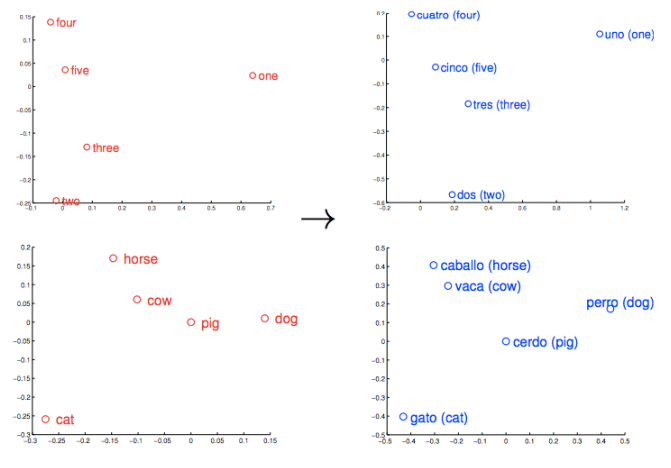
\includegraphics[width=.75\linewidth]{word2vec_translation.png}
	\caption[bla.]{Two examples of distances extracted from word vectors from English and Spanish texts. The top shows the mappings of words of numbers until five and the bottom one of different animals. Interestingly, even word2vec is not trained with any specific language grammar, is able to male similarities among the two languages.}
	\label{fig:lap}
\end{figure}



\section{Related Work}
\label{sec:basics}
First approaches to sentiment and mood mining were relying on basic assumptions. In \cite{Pang} they do a comprehensive review of the more useful techniques for information retrieval.  In \cite{Yang} they infer mood from web blogs using SVM and CRF techniques. It is interesting how taking the assumption of relying on the last sentence of the post gives better accuracy for sentiment prediction. Since relevance of web blogs has decayed, in \cite{Pak}, they do sentiment analysis for tweets. Again, it is different from our scenario since microblogging can take only up to 140 characters and in our case, we have freedom from the reviewer. However, they reach around 80$\%$ accuracy using a bi-gram model and a Naive Bayes classifier. More novel approaches can be found in \cite{Noguishe} where neural architectures (CNN) are applied to the same twitter task with an accuracy of 86,4$\%$ using Stanford Twitter Sentiment from Stanford University. It is also worth to mention that the developed tasks proceed from a Kaggle competition \cite{Kaggle}. In that challenge, the top accuracy scores get to 97$\%$ of accuracy. 


\section{Models/Approaches/Methods Descriptions}
\label{sec:model}


For our analysis, we implemented three different approaches to solve the problem of classification. Thus, we compare three different solutions all by using neural architectures. We used Python with Keras backend to train our models. Consisting of a Multi-Layer Perceptron (MLP), a Convolutional Neural Network (CNN) and a long short-time memory (LSTM).
To load the data we use the already built-in Keras function to import the IMDB corpus. The reviews have been already preprocessed and words are indexed to its number of occurrence in the corpus. We set the maximum of words up to $5000$ and a maximum review length to $500$ words.
For the embedding vector, we also use a built-in Keras function to train it. We specify an output length of $32$, resulting in a $500$ times $32$ embedding vector. The default Keras function works similarly to word2vec. The difference is that with the Keras embedding layer we try to minimize the loss function. On the other hand, word2vec gives an embedding vector that keeps the semantic relation between words. Consequently, the embedding Keras vector might be useful for capturing only polarity of emotions. Nevertheless, the idea still keeps similar for both approaches. 
\subsection{Multi Layer Perceptron}
One of the most simple existing artificial neural networks. Nonetheless, it is known that works as good as other more complex architectures with simple tasks. Since we are dealing with a binary classification problem, it is a good candidate for having good results using less computational resources than other approaches. In our scenario, we have created an MLP with $250$ fully connected neurons with a rectified linear unit (ReLU) activation function. Detailed visualization of the structure of the model can be seen in Figure \ref{fig:mlp}.

\begin{figure}[tbh!]
	\centering
	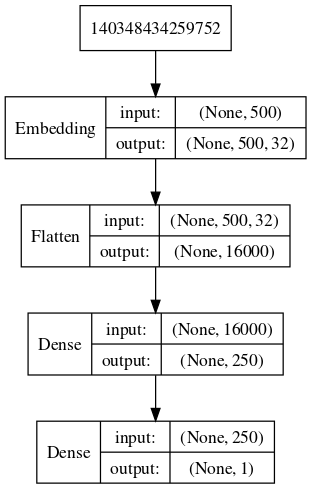
\includegraphics[width=.4\linewidth]{model_MLP.png}
	\caption[bla.]{A detailed structure of the MLP proposed solution. We first get the embedding vectors, then we flatten the vector to input to the fully connected layer and finally, we get the binary classification.}
	\label{fig:mlp}
\end{figure}


\subsection{Convolutional Neural Network}
Convolutional neural networks are interesting neural architectures that can learn features from our data vectors. CNN's have been proven to overcome many other neural architectures in terms of accuracy, specifically in the vision research field. The typical CNN architecture consists of a convolution layer, where a linear convolution is applied to the input, with a certain kernel size. A max pooling layer is added to the architecture to reduce the size of the convolution. Moreover, a fully connected layer is appended to get a classification outcome. The convolution and max-pooling layers can be added arbitrarily to the network to get to a certain vector size. In our case, we only add one time the layers. Therefore, in Figure \ref{fig:cnn} we can see how our architecture looks like.  We use $32$ filters and a $3x3$ kernel size for the convolution layer. The activation function is again ReLU. For the max-pooling layer, we reduce our size by a factor of $2$. Then we add a fully connected layer of $250$ neurons along with the last binary classification.

\begin{figure}[tbh!]
	\centering
	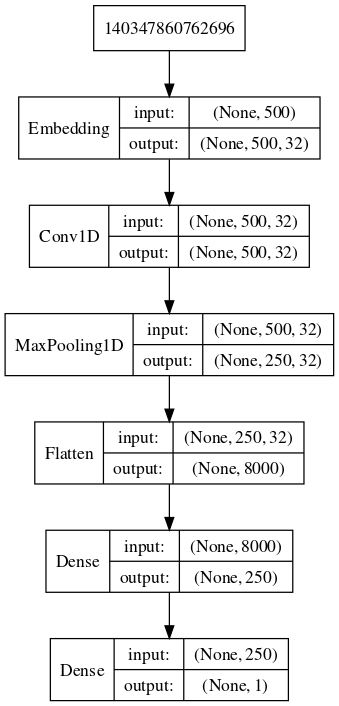
\includegraphics[width=.4\linewidth]{model_CNN.png}
	\caption[bla.]{A detailed structure of the CNN proposed solution. As before, we start with the embedding vector, then we add the one-dimensional convolution operator layer that has the same input size as the embedding vector. The convolution operations return an equally sized matrix. Then we add the sub-sampling or max-pooling layer that reduces our feature space by two. The subsequent part is identical to the MLP model.}
	\label{fig:cnn}
\end{figure}

\subsection{Long Short-Time Memory Network}
LSTM networks are a type of recurrent neural network (RNN) very used in the natural language processing field. They can learn more long-term dependencies than a simple RNN. Since we are working with texts that are longer than a sentence, LSTM is also a good candidate. In Figure \ref{fig:lstm} we can see a detailed explanation of the architecture used. We use $n=100$ as the dimensionality of the output space. \\

\begin{figure}[tbh!]
	\centering
	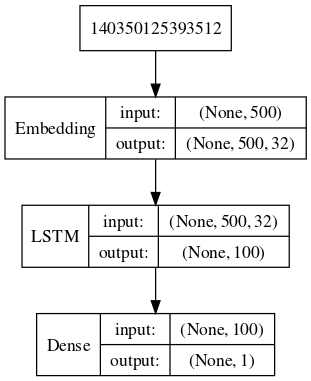
\includegraphics[width=.4\linewidth]{model_LSTM.png}
	\caption[bla.]{Detailed structure of the LSTM architecture used.}
	\label{fig:lstm}
\end{figure}
In each of the above models, we need to add a last layer into the network. The output layer is responsible for classifying between negative and positive reviews, thus consist of only one neuron. The loss function of our models is the binary cross entropy and as a metric, we are interested in the accuracy of the trained model. 


\section{Results/Analysis}
\label{sec:analysis}

\textit{To be written \dots}

\section{Conclusion}
\label{sec:concl}

\textit{To be written \dots}

% insert your bibliographic references into the bib.bib file
%\bibliographystyle{plain}
%\addcontentsline{toc}{section}{Bibliography}% Add to the TOC
\bibliographystyle{unsrt}
\bibliography{kpis_bib}



%\bibliography{kpis_bib}
\end{document}
